\documentclass[12pt]{article}

\usepackage{sbc-template}
\usepackage{amsfonts}
\usepackage{amsmath}
\usepackage{graphicx,url}
\usepackage{comment}
\usepackage[linesnumbered,ruled,vlined,portuguese]{algorithm2e}

\usepackage[brazil]{babel}
%\usepackage[latin1]{inputenc}
\usepackage[utf8]{inputenc}
% UTF-8 encoding is recommended by ShareLaTex


\sloppy

\title{Aplicação de Paralelismo na Resolução do Problema da Soma dos Subconjuntos}

\author{Fernando Concatto\inst{1}}


\address{Bacharelado em Ciência da Computação -- Universidade do Vale do Itajaí (UNIVALI) \\
  Caixa Postal 360 -- CEP 88302-202 -- Itajaí -- SC -- Brasil
  \email{fernandoconcatto@edu.univali.br}
}

\begin{document}

\maketitle

\begin{resumo}
  O Problema da Soma dos Subconjuntos é um problema computacionalmente difícil, demandando tempo exponencial para ser resolvido. Este trabalho buscou aplicar técnicas de processamento paralelo na busca de soluções para o problema, com a intenção de identificar o ganho de desempenho por thread utilizada em comparação com um algoritmo sequencial. Através da análise dos dados experimentais, foi possível constatar que duas threads ofereceram um desempenho aproximadamente duas vezes melhor, enquanto quatro threads ofereceram um desempenho três vezes melhor.
\end{resumo}


\section{Introdução} \label{sec:intro}

Um problema computacional pode ser interpretado como uma questão a ser respondida, geralmente possuindo \textit{parâmetros}, ou \textit{variáveis}. O problema deve ser definido a partir da descrição de todos os seus parâmetros e do estabelecimento de quais propriedades a resposta ou \textit{solução} deve ser composta para ser considerada uma resposta válida para o problema. Uma \textit{instância} do problema é obtida ao atribuir valores a todos os seus parâmetros \cite{Garey1979}.

Algoritmos são procedimentos passo-a-passo que resolvem problemas. Dado um problema, um algoritmo \textit{resolve} tal problema se ele sempre produz uma solução para qualquer uma de suas instâncias. Um objetivo bastante comum na busca de soluções para um problema é o desenvolvimento de um algoritmo eficiente, que resolve o problema no menor tempo possível. O campo da Teoria da Complexidade Computacional busca estudar e classificar os algoritmos, identificando a quantidade de recursos computacionais necessária para executar um algoritmo. Geralmente, a eficiência de um algoritmo é definida pela quantidade de operações fundamentais que o mesmo demanda para resolver o problema. Esta quantidade é usualmente estabelecida em termos do tamanho da instância do problema, que é denotado pelo símbolo $n$ \cite{Arora2009,Garey1979}.

Uma das principais classes de problemas identificadas pela Teoria da Complexidade é a classe NP-completo, um subconjunto da classe NP, que significa \textit{polinomial não determinístico}. A classe NP contém todos os problemas cujas soluções podem ser verificadas em tempo polinomial, enquanto a classe NP-completo é composta por problemas onde todos os problemas em NP podem ser reduzidos para eles em tempo polinomial \cite{Garey1979}. Redução, nesse contexto, significa transformar um problema em outro de forma com que uma solução para o segundo problema também possa ser utilizada para resolver o primeiro \cite{Sipser1996}. Uma classe adicional de problemas estabelecida pela Teoria da Complexidade é a classe P, de \textit{polinomial}; esta classe contém problemas que podem ser solucionados em tempo polinomial ou inferior. P é um subconjunto de NP.

O conceito de tempo polinomial é fundamental para compreender a importância das diferentes classes de problemas. Na tentativa de descrever qual propriedade torna um algoritmo eficiente, pesquisadores propuseram que algoritmos que demandavam uma quantidade de operações exponencial em relação ao tamanho do problema ($n$) eram excessivamente ineficientes, devido ao fator de crescimento multiplicativo. Desta forma, algoritmos eficientes foram definidos como possuindo um tempo de execução polinomial, isto é, demandando no máximo $n^{k}$ operações, onde $k$ é uma constante \cite{Kleinberg2005}. A figura \ref{fig:complexity} demonstra uma comparação entre alguns fatores de crescimento bastante comuns, evidenciando a velocidade do crescimento da quantidade de operações exigidas por algoritmos de tempo exponencial, denotada pela curva laranja (segunda à esquerda).

\begin{figure}[ht]
    \centering
    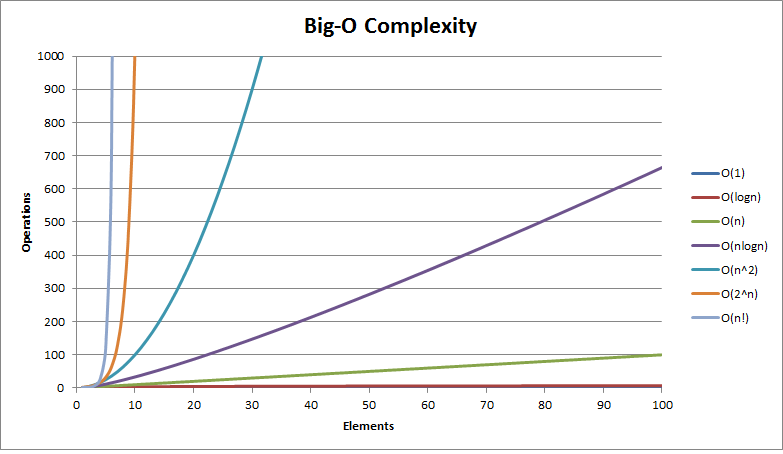
\includegraphics[width=13cm]{complexity.png}
    \caption{Comparação entre a quantidade de operações fundamentais em função do tamanho do problema.}
    \label{fig:complexity}
\end{figure}

Apesar de que as soluções para problemas NP-completos podem ser verificadas em tempo polinomial, nenhum algoritmo para resolver um problema NP-completo em tempo polinomial foi encontrado até hoje; todos demandam tempo exponencial ou superior. Apesar disso, não há nenhuma prova de que não existe um algoritmo eficiente para resolver problemas NP-completos. Esta condição é um dos principais pontos da questão ``P $=$ NP?'', um dos maiores problemas abertos no campo da Ciência da Computação \cite{Sipser1996}.

Entre os problemas pertencentes à classe NP-completo está o Problema da Soma dos Subconjuntos. Sua NP-completude foi comprovada por Richard Karp, juntamente com diversos outros problemas, em seu artigo de 1972, intitulado ``Reducibility Among Combinatorial Problems'' \cite{Karp1972}. Por ser um problema NP-completo, não se conhece um algoritmo capaz de resolvê-lo em tempo polinomial. Este trabalho se propôs a analisar este problema aplicando técnicas de processamento paralelo, com a intenção de acelerar a velocidade de busca pela solução do problema utilizando um algoritmo de força bruta, que demanda tempo exponencial, e analisar o ganho de desempenho obtido em função da quantidade de unidades de processamento executando simultaneamente.

\section{Definição do problema} \label{sec:def}

O Problema da Soma da Soma dos Subconjuntos, como especificado por \cite{Garey1979} a partir de uma transformação do problema ``Knapsack'' de Richard Karp, é definido da seguinte forma: dado um conjunto $A = \left\{a \mid a \in \mathbb{Z}^{+}\right\}$ e um número inteiro $b$, existe um subconjunto $A' \subseteq A$ onde a soma de todos os elementos de $A'$ é exatamente $b$?

No escopo deste trabalho, o problema será ligeiramente simplificado com a intenção de facilitar sua análise no contexto de processamento paralelo. O parâmetro $b$ será tratado como 0, e consequentemente, os valores do conjunto $A$ pertencerão a $\mathbb{Z}$ (isto é, poderão ser negativos ou zero) e $\left | A' \right | > 0$ (ou seja, o subconjunto não poderá ser vazio). Desta forma, o Problema da Soma dos Subconjuntos será tratado da seguinte forma:

\begin{equation} \label{eq:subsetsum}
    \sum_{i = 1}^{n} a_{i} x_{i} = 0
\end{equation}

Onde $a_{i} \in A$, $x_{i} \in \left\{0, 1\right\}$ e $\sum x_{i} > 0$. Um algoritmo que resolve este problema deve determinar se existe uma sequência de valores de $x$ que soluciona a equação \ref{eq:subsetsum}. Esta formulação é equivalente a encontrar um subconjunto não-vazio de $A$ cuja soma é igual a zero. Utilizando técnicas de análise combinatória, é possível estabelecer que a quantidade de possíveis sequências de $x$ é igual a $2^{n} - 1$, onde $n = \left | A \right |$. Este valor é equivalente à quantidade de subconjuntos não-vazios de um conjunto qualquer, definida por:

\begin{equation} \label{eq:subsetcount}
    \sum_{k = 1}^{n} \binom{n}{k} = 2^{n} - 1
\end{equation}

O algoritmo aplicado neste trabalho tentará verificar todas as combinações de $x$ até que encontre uma combinação que solucione a equação ou até que as combinações se esgotem. Portanto, o algoritmo irá demandar tempo exponencial, pois no pior caso, todas as $2^{n} - 1$ combinações deverão ser testadas.

\section{Trabalhos relacionados} \label{sec:relatedwork}

O Problema da Soma dos Subconjuntos é um objeto de estudo frequente no campo da criptoanálise. Devido à inexistência de algoritmos exatos eficientes para resolver este problema, alguns criptossistemas baseados em suas propriedades foram desenvolvidos.

O criptossistema de \cite{Merkle1978} envolve a utilização de um problema derivado do Problema da Soma dos Subconjuntos, conhecido como \textbf{problema da mochila}, onde cada elemento do conjunto é composto por um peso e uma quantidade. Este trabalho explora instâncias particularmente difíceis do problema da mochila, que entretanto podem ser resolvidas facilmente através do conhecimento de certas propriedades do conjunto de pesos da instância; estas propriedades são chamadas de \textit{trapdoor information}. O sistema foi um dos pioneiros na utilização de conceitos de criptografia assimétrica, porém sua segurança não pôde ser comprovada, devido à ausência de provas concretas da dificuldade computacional de problemas NP-completos.

A proposta de criptossistemas baseados no problema da mochila foi respondida com diversas pesquisas sobre técnicas eficientes para quebrá-los. Um destes trabalhos, desenvolvido por \cite{Lagarias1985}, utiliza uma transformação do problema da mochila para a busca por um vetor curto em um reticulado (\textit{lattice}), posteriormente aplicando um algoritmo de tempo polinomial para tentar resolvê-lo. A técnica se mostrou bastante eficiente, entretanto nem sempre foi capaz de encontrar a solução em casos onde os pesos do conjunto eram codificados com um número elevado de bits.

\section{Processamento paralelo} \label{sec:parallel}

Para realizar a execução do algoritmo em mais de uma unidade de processamento simultaneamente, o conceito de \textit{multithreading} foi aplicado. \textit{Thread} é um conceito abstrato que descreve a sequência de execução de um programa, ou o trabalho sendo realizado pelo computador. Threads são similares à processos, porém são entidades muito mais leves, que carregam apenas informações dos registradores, da pilha e alguns outros dados, enquanto processos contém diversas outras informações, como mapas de memória, \textit{file descriptors} e o código e dados do programa propriamente dito. Todas essas informações que compõem um processo são compartilhadas entre suas threads, cuja quantidade pode variar de apenas uma para múltiplas por processo \cite{Lewis1996}.

Crucialmente, todas as threads de um processo podem acessar o código e os dados daquele programa. Desta forma, as threads podem executar qualquer subrotina globalmente visível no programa; o mesmo é aplicável no acesso à variáveis. Portanto, threads podem cooperar na resolução de problemas, desde que o mesmo possa ser dividido em múltiplos subproblemas independentes, para que possam ser executados paralelamente pelas threads. Com isso, desconsiderando o impacto dos procedimentos de divisão de trabalho, espera-se que um problema sendo resolvido paralelamente por $n$ threads seja solucionado em $n$ vezes menos tempo do que sua versão sequencial.

\section{Experimentos} \label{sec:experiments}

Para a realização dos experimentos, foi escrito um programa  na linguagem C utilizando a biblioteca POSIX Threads (\textit{pthreads}) para realizar a divisão do trabalho entre múltiplas threads. Os experimentos foram executados conforme os seguintes parâmetros:

\begin{itemize}
    \item Quantidade de threads, com valores 1, 2 e 4;
    \item Tamanho do conjunto ($n$), variando de 4 a 52 com incrementos de 4;
    \item Quantidade de bits dos valores no conjunto, dada pela expressão $2^{0.5n}$.
\end{itemize}

Para os experimentos envolvendo múltiplas threads, um parâmetro adicional foi estabelecido para definir a quantidade de subconjuntos que cada thread deve testar ininterruptamente. Este parâmetro foi chamado de \textit{tamanho do trabalho}, e recebeu como valores 10, 100 e 1000.

\begin{algorithm}[ht]
  \small
  \DontPrintSemicolon
  \caption{Problema da Soma dos Subconjuntos em Paralelo}
  \label{alg:exp}
  \SetKwInOut{Input}{Entrada}
  \SetKwInOut{Output}{Saída}
  \SetKwBlock{Parallel}{Paralelamente em}{}
  \Input{$n, bits, nThreads, trabalho$}
  \Output{$solucao, duracao$}

  \BlankLine
  $inicio \leftarrow tempo()$ \;
  $conjunto \leftarrow gerarConjuntoAleatorio(n, bits)$ \;
  $threads \leftarrow criarIdentificadores(nThreads)$ \;
  \BlankLine
  \ForEach{thread $\in$ threads} {
    \Parallel($thread$){
        \While{houver trabalho e término não for sinalizado} {
            $inicio \leftarrow obterTrabalho(trabalho)$ \;
            \For{i = inicio \emph{\KwTo} inicio + trabalho} {
                \If{i $\geq 2^{n} - 1$}{
                    \tcp{subconjuntos esgotados}
                    $finalizarThread(thread, \emptyset)$ \;
                }
                $subconjunto \leftarrow gerarSubconjunto(conjunto, i)$ \;
                $soma \leftarrow somarElementos(subconjunto)$ \;
                \BlankLine
                \If{soma = 0}{
                    $sinalizarTermino()$ \;
                    $finalizarThread(thread, subconjunto)$ \;
                }
            }
        }
        \BlankLine
        $finalizarThread(thread, \emptyset)$ \;
    }
    \BlankLine
    $iniciarExecucao(thread)$ \;
  }
  \BlankLine
  $solucao \leftarrow \emptyset$ \;
  \BlankLine
  \ForEach{thread $\in$ threads} {
    $resultado \leftarrow aguardarExecucao(thread)$ \;
    \If{$resultado \neq \emptyset$} {
      $solucao \leftarrow resultado$ \;
    }
  }
  \BlankLine
  $duracao \leftarrow tempo() - inicio$ \;
  \Return{$\{solucao, duracao\}$} \;
\end{algorithm}

O procedimento utilizado na realização dos experimentos em paralelo é definido pelo algoritmo \ref{alg:exp}, através de uma representação em pseudocódigo; a seguir, suas particularidades serão descritas. Como entrada, o algoritmo recebe o tamanho do conjunto $n$, a quantidade de bits dos valores do conjunto, a quantidade de threads e o tamanho do trabalho. Inicialmente, o tempo atual é gravado para calcular a duração do algoritmo. Em seguida, um conjunto é gerado aleatoriamente com base nos parâmetros recebidos. Então, os identificadores das threads são criados para controlá-las durante a execução do programa. Na sequência, as operações que serão executadas em paralelo são especificadas.

Cada thread permanece em um \textit{loop} que executa até que todos os subconjuntos sejam testados ou até que alguma thread encontre uma solução, realizando as operações detalhadas a seguir. O ponto de partida do trabalho é gerado pela função \textit{obterTrabalho}, que mantém o estado atual do trabalho, partindo do número 1 e sendo incrementado pelo parâmetro \textit{trabalho}. O estado deve ser protegido por uma \textit{mutex}, pois será acessado por várias threads; caso contrário, uma condição de corrida poderia ocorrer, causando anomalias no valor do estado \cite{Lewis1996}.

Em seguida, um loop é iniciado partindo do ponto gerado pelo procedimento descrito anteriormente e executando \textit{trabalho} vezes. Para cada iteração do loop, um subconjunto é gerado a partir da representação em binário do estado atual (por exemplo, no estado 7$_{10}$ = 111$_{2}$, apenas os três primeiros elementos do conjunto original serão inclusos). Caso o valor do estado atual ultrapasse a quantidade de subconjuntos, a thread é finalizada com o conjunto vazio como resultado. Caso contrário, a soma dos elementos do subconjunto é computada e, caso seja zero, todas as threads serão sinalizadas para interromperem sua execução e a thread atual será finalizada com o subconjunto atual como resultado. Por fim, caso todos os subconjuntos já tiverem sido testados, a thread termina com o conjunto vazio como resultado.

Enquanto as threads buscam a solução para o problema, o programa principal declara a solução final, inicialmente vazia, e fica aguardando o término das threads. Cada uma delas conterá um resultado, indicado pelas chamadas da função \textit{finalizarThread}. Caso o resultado de uma thread seja o conjunto vazio, a solução fica inalterada; caso contrário, a solução recebe o subconjunto que a thread encontrou. Quando todas as threads forem finalizadas, o algoritmo é terminado e retorna a solução encontrada (ou o conjunto vazio se não houver solução) e a duração do procedimento, que é calculada a partir da diferença entre o tempo atual e o tempo inicial.

A versão sequencial do algoritmo é bastante similar à versão paralela, exceto pela ausência das threads. Desta forma, não é necessário criar identificadores, separar o trabalho em blocos, nem iniciar, sincronizar e aguardar o término das threads. O valor cuja representação em binário indica o subconjunto a ser gerado é simplesmente inicializado em 1 e incrementado a todo momento em que a solução não é encontrada, até atingir $2^{n} - 1$.

Os experimentos foram realizados em um computador com processador Intel Core i3-3240 com clock de 3.4 GHz e 4 núcleos e com o sistema operacional Windows 10 Pro 64 bits. O programa foi compilado utilizando GCC versão 4.8.1 no ambiente MinGW. Um aspecto importante para melhorar a confiabilidade dos dados foi estabelecer a mesma \textit{seed} para o gerador de números aleatórios nos diferentes testes, fazendo com que as sequências de valores gerados para os conjuntos sejam idênticas. Cada teste foi composto por 30 execuções do algoritmo para cada tamanho de conjunto.

\section{Análise dos resultados} \label{sec:results}

O primeiro passo tomado para analisar os resultados obtidos foi investigar as diferenças entre os distintos tamanho de trabalho para duas e quatro threads, observando qual tamanho de trabalho oferece o melhor desempenho, mensurado pela média de tempo entre todos os tamanhos de conjunto. Esta análise é apresentada na figura \ref{fig:chunks}, através da qual foi possível perceber que a diferença de desempenho é bastante pequena, porém o tamanho de trabalho 1000 se mostrou superior aos outros para quatro threads e ligeiramente inferior a 100 para duas threads.

\begin{figure}[ht]
    \centering
    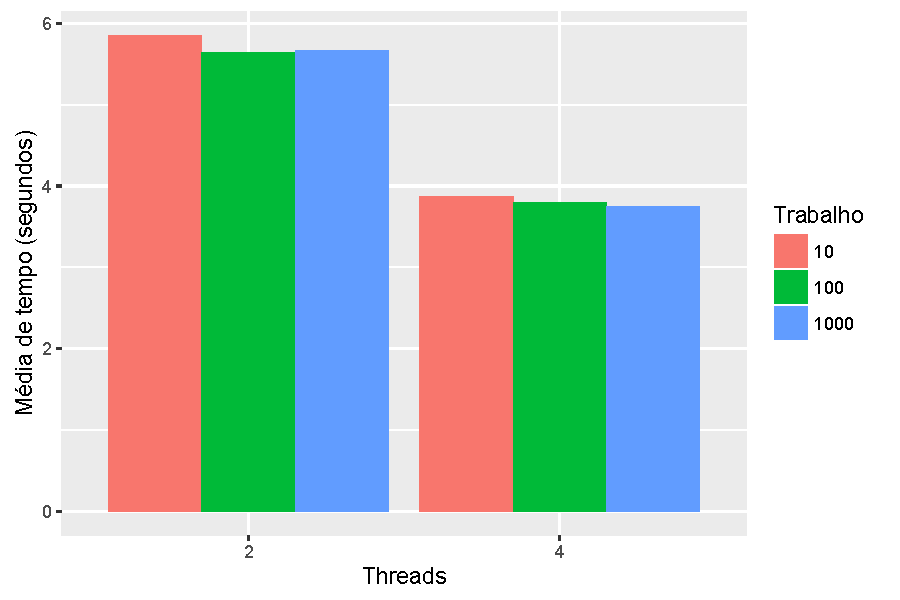
\includegraphics[width=9cm]{chunks}
    \caption{Média de tempo para diferentes tamanhos de trabalho}
    \label{fig:chunks}
\end{figure}

Um aspecto interessante deste resultado é a tendência a uma performance melhor com 4 threads enquanto o tamanho do trabalho aumenta. Um trabalho futuro poderia investigar a efetividade de tamanhos de trabalho ainda maiores.

Com isso, o tamanho de trabalho 1000 será utilizado nas análises a seguir. O próximo passo efetuado foi a realização da principal proposta deste trabalho: analisar o ganho de desempenho em função da quantidade de threads utilizadas. O gráfico da figura \ref{fig:performance} apresenta as médias de tempo que o algoritmo demandou para solucionar o problema em função do tamanho do conjunto, para 1, 2 e 4 threads. É possível perceber um ganho significativo de performance, especialmente quando $n > 40$.

\begin{figure}[ht]
    \centering
    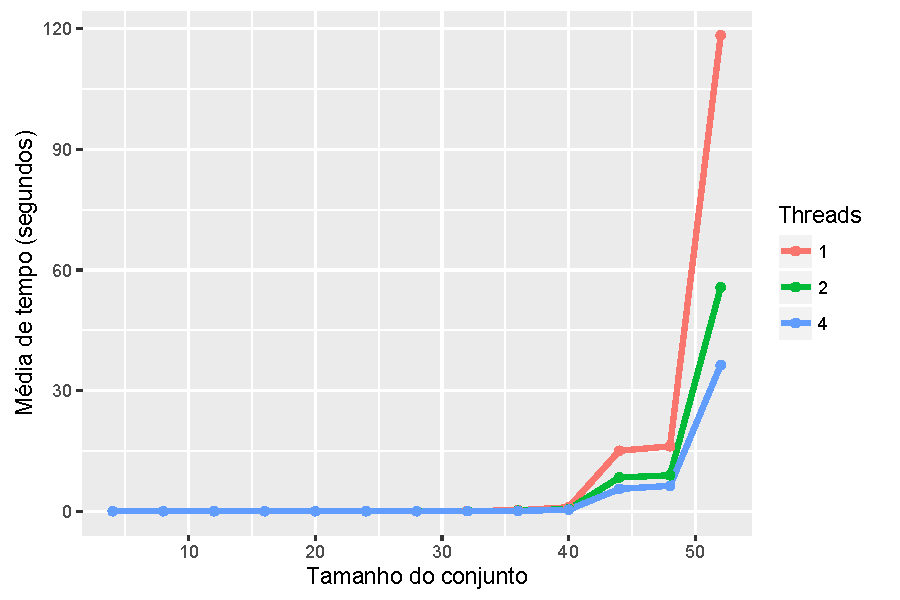
\includegraphics[width=10cm]{performance}
    \caption{Média de tempo em função do tamanho do conjunto (n) para diferentes quantidades de threads}
    \label{fig:performance}
\end{figure}

Para visualizar detalhadamente o ganho de performance, os dados foram dispostos de forma tabular na tabela \ref{tab:speedtable}. As durações apresentadas foram calculadas a partir da média de duração de todas as 30 iterações.

\begin{table}[ht]
    \centering
    \caption{Tempo médio consumido pelo algoritmo, em segundos}
    \label{tab:speedtable}
    \smallskip

    \begingroup
    \renewcommand*{\arraystretch}{1.2}

    \begin{tabular}{|c|r|r|r|}
        \hline
        \textbf{Tamanho do conjunto} & \textbf{Sequencial} & \textbf{2 threads} & \textbf{4 threads} \\
        \hline
        44 & 15.051 & 8.413 & 5.559 \\
        \hline
        48 & 16.152 & 8.943 & 6.333 \\
        \hline
        52 & 118.415 & 55.673 & 36.352 \\
        \hline
    \end{tabular}

    \endgroup

\end{table}

Através da tabela \ref{tab:speedtable} é possível observar uma melhora significativa nos tempos de execução do algoritmo. Realizando o cálculo de ganho de desempenho, os seguintes valores foram descobertos:

\begin{itemize}
    \item Melhora de 1.79 vezes para duas threads e 2.71 vezes para quatro threads, quando $n = 44$;
    \item Melhora de 1.81 vezes para duas threads e 2.55 vezes para quatro threads, quando $n = 48$;
    \item Melhora de 2.13 vezes para duas threads e 3.26 vezes para quatro threads quando $n = 52$.
\end{itemize}

Efetuando a média aritmética dos valores encontrados, é possível estabelecer que o tempo de execução para duas threads foi 1.91 vezes mais veloz, enquanto para quatro threads a melhora é de 2.84 vezes.

\section{Conclusões} \label{sec:conclusions}

As análises descritas neste trabalho foram realizadas com a intenção de investigar a melhora de desempenho proporcionada por processamento paralelo, utilizando o Problema da Soma dos Subconjuntos como contexto para os testes. Através do estudo dos dados experimentais coletados, foi possível observar um ganho de performance ligeiramente menor, porém não muito distante do resultado esperado, quando o algoritmo é executado paralelamente.

Utilizando duas threads, a melhora no desempenho foi bastante significativa, até mesmo ultrapassando o resultado esperado para o maior tamanho de conjunto testado (52). Entretanto, para quatro threads, esperava-se observar uma melhora de quatro vezes no tempo consumido pelo algoritmo, porém o resultado obtido permaneceu em torno de três. É bastante provável que essa diferença seja causada pelo \textit{overhead} produzido pelo processador para gerenciar a execução de múltiplas de threads, especialmente porque todos os quatro núcleos do processador empregado nos testes estavam operando em utilização máxima.

Por fim, foi possível também observar claramente a dificuldade computacional de um problema NP-completo. Mesmo com a utilização de quatro threads, conjuntos de 52 elementos já demandavam tempo de execução bastante elevado, em torno de 36 segundos. Além disso, visualizando o gráfico da figura \ref{fig:performance}, o crescimento exponencial de tempo necessário para resolver o problema fica bastante evidente. Desta forma, conclui-se que apesar de fornecer um ganho de desempenho considerável, o processamento paralelo não é páreo para a complexidade de problemas NP-completos.

\bibliographystyle{sbc}
\bibliography{sbc-template}

\end{document}
